\chapter{INTRODUCTION}\label{chap:intro}

\section{Biosecurity and Policies}

The global community is grappling with an escalating array of biological threats that cut across national borders, economic sectors, and scientific disciplines. The COVID-19 pandemic laid bare just how devastating these threats can be, claiming millions of lives and inflicting trillions of dollars in economic damage \citep{WHO2021, Hulme2021}. In today's interconnected world---where rapid international travel and sprawling trade networks are the norm---biological threats can spread at alarming speed. Responding effectively demands coordinated action that weaves together public health measures, border controls, surveillance systems, and emergency management protocols \citep{WTO2024}.

The World Health Organization defines biosecurity as a strategic and integrated approach to analyzing and managing risks to human, animal, and plant life and health, along with associated environmental risks \citep{WHO2021}. This broad perspective acknowledges the deep connections among human health, animal health, plant health, and ecosystem integrity---what is often called the One Health approach \citep{Hulme2021}. The Food and Agriculture Organization similarly emphasizes that biosecurity encompasses the policy and regulatory frameworks needed to analyze and manage risks in food safety, animal welfare, and plant protection \citep{FAO2023}. Making biosecurity work in practice requires coordination across a wide range of sectors: agriculture, veterinary medicine, public health, environmental protection, customs and border control, transportation, and---increasingly---information technology and cybersecurity.

Biosecurity governance rests on a complex architecture of international agreements and national regulations. At the global level, the World Health Organization's International Health Regulations create binding obligations for member states to build core capacities for detecting, assessing, reporting, and responding to public health emergencies \citep{WHO2021}. Bodies such as the World Organisation for Animal Health and the Codex Alimentarius Commission develop standards that member states draw on when managing biosecurity risks \citep{WTO2024}. Meanwhile, the Biological Weapons Convention prohibits the development, production, and stockpiling of biological weapons, establishing a normative foundation against the harmful use of biological agents \citep{UNODA2023}.

Malaysia has put in place comprehensive biosecurity policies that reflect both its exposure to biological threats and its strategic position in global trade. As a tropical country with extensive agricultural production and major exports of commodities like palm oil and rubber, Malaysia faces biosecurity risks from endemic diseases, imported pests and pathogens, and the possibility of bioterrorism \citep{Malaysia2023}. Its location along the Strait of Malacca---through which roughly one-quarter of global maritime trade passes---makes it a critical node in international supply chains and a potential gateway for biological threats \citep{ASEAN2024}.

Recognizing how central cybersecurity has become to national security and economic competitiveness, Malaysia enacted the Cybersecurity Act 2024, which came into force on 26 August 2024 \citep{Malaysia2024}. This landmark legislation sets up a comprehensive framework for managing cybersecurity risks to critical information infrastructure, including systems that support biosecurity functions. The Act designates the National Cyber Security Agency as the lead authority for coordinating cybersecurity policy and incident response, with powers to designate systems as National Critical Information Infrastructure and to require their operators to adopt cybersecurity measures, report incidents, and undergo regular audits \citep{NACSA2024}. Notably, the legislation reaches beyond national borders to cover cybersecurity service providers whose activities affect Malaysia's cybersecurity posture, reflecting the inherently cross-border nature of cyber threats \citep{CMS2024}.

Malaysia has also established regulatory frameworks for unmanned aerial systems. The Civil Aviation Authority of Malaysia enforces comprehensive drone regulations under the Malaysian Civil Aviation Regulations 2016, which categorize unmanned aircraft by weight and operational characteristics \citep{CAAM2024}. Small Unmanned Aircraft Systems weighing up to 20 kilograms face relatively flexible regulations for recreational use, while commercial operations require permits with specific requirements for operator qualifications, aircraft certification, and insurance coverage \citep{DroneAcademy2023}. Several locations have been designated as no-fly zones for security purposes, including Putrajaya, the Kuala Lumpur City Centre, Parliament House, and military installations \citep{DroneRegulations2024}.

Biosecurity spans multiple interlinked domains, each addressing a different category of biological threat. Agricultural biosecurity protects crops, livestock, and aquaculture from pests and diseases through quarantine inspections, certification programs, pest surveillance, and rapid response protocols \citep{FAO2023}. Public health biosecurity tackles infectious disease threats to human populations through disease surveillance systems, laboratory networks, stockpiles of medical countermeasures, and health system surge capacity \citep{WHO2021}. Environmental biosecurity safeguards ecosystems and biodiversity from invasive alien species and genetically modified organisms \citep{Hulme2021}. Laboratory biosecurity ensures the secure storage and handling of dangerous pathogens through biosafety regulations and inventory management.

Figure \ref{fig:biosecurity_types} illustrates the major types of biosecurity and their relationships, with particular emphasis on the central role that cybersecurity plays in enabling and protecting biosecurity functions across all domains.

\begin{figure}[htbp]
	\centering
	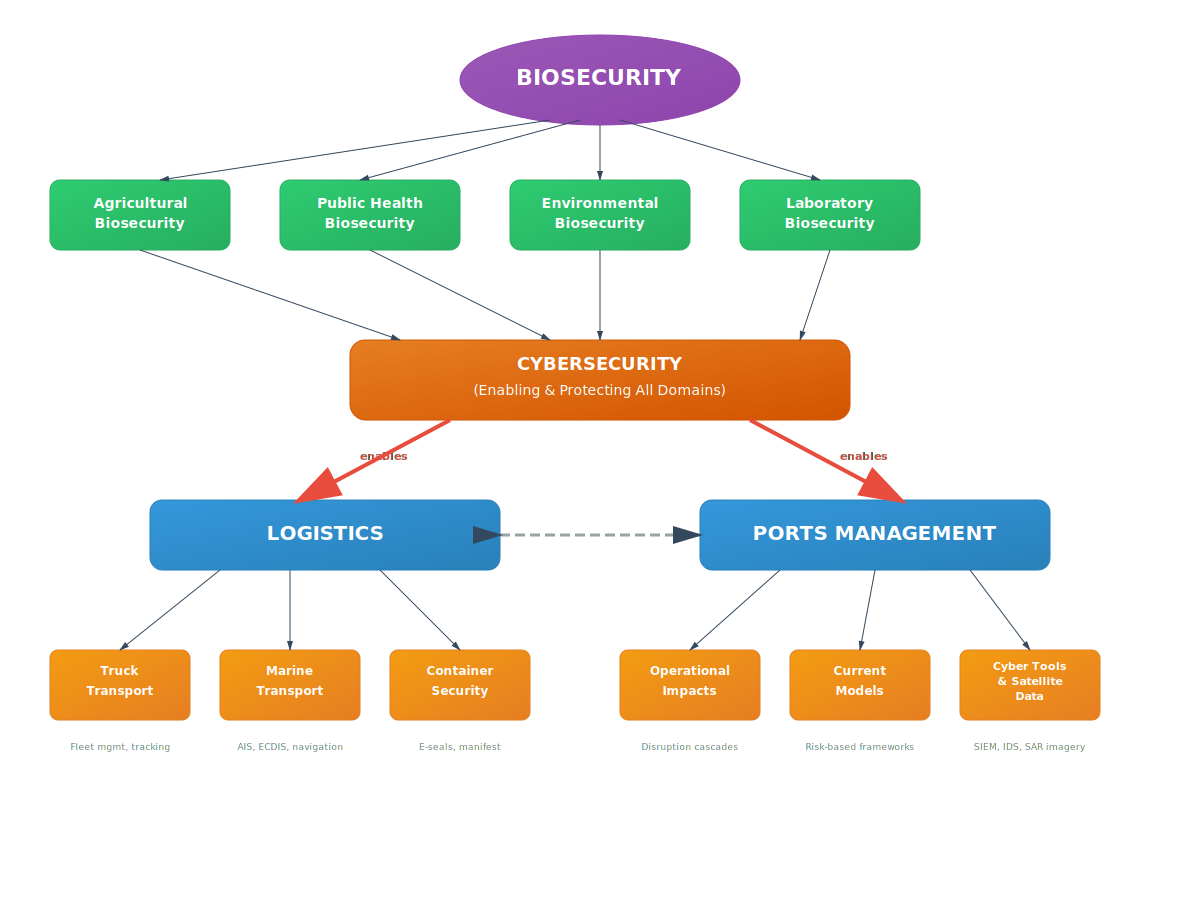
\includegraphics[width=0.90\textwidth]{figures/biosecurity_types_framework.png}
	\caption{Types of Biosecurity and the Central Role of Cybersecurity}
	\label{fig:biosecurity_types}
\end{figure}

Within this broader landscape, cybersecurity has emerged as a critical enabling capability that underpins the effectiveness of biosecurity measures across every domain. Modern biosecurity systems depend heavily on digital technologies for surveillance, data management, communication, laboratory analysis, and coordination of response activities \citep{ENISA2023}. Disease surveillance systems collect and analyze vast quantities of data from healthcare facilities and laboratories to catch outbreaks early and track their spread. Border control systems use databases, risk assessment algorithms, and electronic cargo tracking to target inspections at high-risk shipments while keeping legitimate trade flowing. Laboratory information management systems maintain inventories of dangerous pathogens and track specimen transfers. Emergency management systems coordinate the deployment of personnel and resources during outbreaks. All of these digital systems create dependencies on cybersecurity---their compromise could blind surveillance networks to emerging threats, misdirect response resources, or even enable the theft of dangerous pathogens.

Cybersecurity intersects with biosecurity through two domains that are vital to global commerce and public health: logistics operations and port management. Modern logistics systems rely on information technologies to coordinate the movement of goods across supply chains that span multiple countries and transportation modes \citep{Notteboom2024}. Truck transportation increasingly employs digital fleet management systems, electronic logging devices, and real-time cargo tracking---technologies that boost operational efficiency but also create cybersecurity vulnerabilities \citep{DHS2024}. Marine transportation has adopted automatic identification systems, electronic chart displays, and satellite communications that improve safety and efficiency while simultaneously creating new attack surfaces for cyber intrusions \citep{IMO2022}. Container shipping depends heavily on digital systems including electronic cargo manifests, automated risk assessment algorithms, electronic seals, and tracking systems that follow goods throughout the supply chain \citep{WCO2023}.

Port management represents a particularly critical nexus of cybersecurity and biosecurity concerns, given that ports serve as gateways for international trade and potential entry points for biological threats. Modern ports function as complex cyber-physical systems that integrate information technology, operational technology, and physical infrastructure \citep{Notteboom2024}. Terminal operating systems coordinate container movements; port community systems facilitate information sharing among organizations; vessel traffic management systems monitor ship movements; and cargo screening technologies enable non-intrusive inspection for contraband, including dangerous biological materials. The 2017 NotPetya ransomware attack on Maersk Line demonstrated just how vulnerable global shipping infrastructure can be, costing approximately 300 million US dollars and forcing the shutdown of 76 container terminals \citep{Lloyd2018}. More recently, the 2023 ransomware attack on the Port of Nagoya forced the suspension of container operations for four days \citep{MarineDigital2023}.

Current operational models for port management increasingly treat cybersecurity as a fundamental component of port security. Leading port authorities have adopted risk-based cybersecurity frameworks aligned with international standards, including the International Maritime Organization's Guidelines on Maritime Cyber Risk Management, the National Institute of Standards and Technology Cybersecurity Framework, and ISO/IEC 27001 \citep{IMO2022, NIST2023, ISO27001}. The tools and technologies deployed for port cybersecurity include network security solutions such as firewalls and intrusion detection systems, industrial control system security for operational technology environments, security information and event management platforms, endpoint detection and response solutions, and vulnerability assessment tools \citep{ENISA2023}.

Terrain and satellite data play an increasingly important role in port security by providing capabilities for monitoring port facilities and tracking vessel movements. Satellite-based automatic identification systems enable global tracking of ship movements for maritime domain awareness and security surveillance \citep{IMO2022}. Synthetic aperture radar satellites provide all-weather imagery of port facilities and surrounding waters, while optical satellite imagery enables detailed monitoring of port infrastructure and vessel identification \citep{ESA2023}. However, reliance on space-based systems introduces potential vulnerabilities if satellite systems are disrupted by technical failures or deliberate attacks \citep{DHS2024}.

This thesis addresses the critical need for efficient, reliable, and secure pathfinding capabilities for autonomous vehicles operating in biosecurity-sensitive environments such as agricultural facilities, healthcare settings, transportation hubs, and border control operations. The research develops novel algorithms for grid-based pathfinding that cut computational complexity while maintaining path quality and enabling real-time responsiveness to dynamic environment changes. Particular attention is paid to risk-aware pathfinding that minimizes exposure to contaminated or high-risk areas---a capability that is essential when autonomous systems operate in biosecurity contexts where human safety and mission effectiveness hinge on avoiding known or suspected hazards.


\section{Problem Statement}

Deploying autonomous systems for grid-based navigation involves several interconnected challenges that limit their effectiveness and practical utility, particularly in time-critical and risk-sensitive applications. This section identifies two key problems that significantly constrain current autonomous navigation capabilities.

\textbf{Problem 1: Real-time Computational Constraints.} Standard pathfinding algorithms hit a fundamental wall when applied to large-scale or highly cluttered environments: computation time grows prohibitively as problem complexity increases. On large grids, the state space expands quadratically with environment dimensions, forcing algorithms to examine vast numbers of potential paths before arriving at acceptable solutions. This computational burden becomes especially severe in risk-annotated grids commonly used for biosecurity applications, where each cell contains not only traversability information but also exposure data that requires evaluation of composite cost functions balancing distance against risk. The problem intensifies in cluttered environments with narrow aisles or complex obstacle configurations, where algorithms must explore numerous alternative routes before finding feasible paths. In time-critical missions---biosecurity surveillance, rapid response to detected contamination, emergency disinfection operations---these computational delays directly undermine mission effectiveness. When autonomous systems cannot compute paths quickly enough to keep pace with evolving situations, the resulting hesitation can compromise operational objectives and potentially endanger human operators or critical assets that depend on timely deployment of autonomous platforms.

\textbf{Problem 2: Limited Adaptability to Dynamic Environments.} Real-world operational environments rarely stay static. Occupancy and risk information change frequently due to moving obstacles, personnel activity, updated sensor readings, new test results, and evolving contamination zones. In biosecurity contexts specifically, risk maps may need updating based on newly detected pathogens, revised quarantine boundaries, or the temporal progression of contamination spread. Current planning approaches struggle with this inherent dynamism. When conditions change, most systems must restart the entire planning process from scratch, discarding all previously computed information. This complete restart incurs substantial computational overhead---a particular problem when updates occur frequently or when environments are large and complex. The delays from repeated full re-planning become critical bottlenecks in time-sensitive scenarios where rapid adaptation is needed to maintain safety margins and mission effectiveness. Beyond raw computational costs, frequent complete re-planning can produce inconsistent or oscillating path selections, potentially confusing human operators who must supervise autonomous operations, or undermining system reliability when paths change dramatically in response to minor environmental updates. The fundamental issue is that current systems lack mechanisms to efficiently update existing plans by incorporating only locally relevant changes. Instead, every environmental modification---however small---is treated as requiring complete plan reconstruction.


\section{Research Questions and Research Hypotheses}

Building on the problems identified in Section 1.2, this research formulates two research questions and corresponding hypotheses that guide the development, implementation, and evaluation of the proposed pathfinding techniques.

\textbf{Research Question 1 (RQ1):} To what extent can constraining search to an Incremental Line Search (ILS) corridor reduce computational requirements and cumulative exposure while preserving path optimality on risk-annotated grid maps?

\textbf{Research Hypothesis 1 (RH1):} The ILS approach will achieve significant reductions in runtime and node expansions (an expected reduction of 40--70\% compared to standard A*) while maintaining path lengths within 5\% of optimal solutions. On risk-annotated grids, ILS will also reduce the cumulative exposure integral (the sum of risk values along the path) by prioritizing paths through the corridor that naturally avoid high-risk regions, with negligible impact on path quality as measured by standard optimality metrics.

\textbf{Research Question 2 (RQ2):} Can an adaptive corridor mechanism that dynamically adjusts ILS corridor width based on local obstructions and risk concentrations support efficient re-planning under dynamic environmental updates while maintaining exposure constraints?

\textbf{Research Hypothesis 2 (RH2):} An adaptive corridor widening strategy that expands the search space only near detected obstructions or risk spikes will sustain the computational advantages of ILS (maintaining 50--80\% of the speedup observed in static scenarios) while successfully handling moderate environment dynamics. The adaptive mechanism will keep cumulative exposure within user-specified thresholds (e.g., no more than 15\% increase in exposure integral) even under dynamic updates, and will achieve re-planning latencies 3--5 times faster than complete re-planning approaches.


\section{Research Objectives}

The overarching aim of this research is to develop, implement, and validate efficient grid-based pathfinding techniques for autonomous systems that combine computational efficiency with practical deployability, particularly in risk-sensitive biosecurity applications. This aim is pursued through two specific research objectives:

\textbf{Objective 1 (O1):} Design and evaluate an Incremental Line Search (ILS) framework for risk-aware pathfinding that focuses exploration within a narrow corridor centred on a direct line between start and goal positions.

\textbf{Objective 2 (O2):} Develop and validate an adaptive corridor control mechanism for ILS that dynamically adjusts corridor width based on local environmental features, including obstacle concentrations and risk-level spikes.


\section{Scope and Limitations}

This research focuses on grid-based pathfinding for autonomous navigation, with specific scope boundaries and acknowledged limitations that define how far the results can be applied and generalized.

\textbf{Environment Representation:} The research considers two-dimensional occupancy grids with optional risk layers. Grid cells are classified as either traversable or occupied, with traversable cells optionally annotated with continuous risk values normalized to [0, 1]. The evaluation encompasses grid sizes from 50$\times$50 to 1000$\times$1000 cells and obstacle densities from 10\% to 40\%. Risk distributions include uniform random patterns, localized hotspots, and structured zones reflecting quarantine areas or contamination gradients. Full three-dimensional environments with varying altitude constraints fall outside the scope of this work.

\textbf{Agent Model:} A single autonomous agent with either 4-connected or 8-connected motion primitives is assumed. For aerial vehicles, a fixed-altitude abstraction is employed. The agent is modeled as occupying a single grid cell at any discrete time step. Vehicle dynamics and continuous-time trajectory optimization are handled at the execution layer rather than in the planning phase. Multi-agent coordination is explicitly excluded.

\textbf{Environment Dynamics:} The research considers moderate, piecewise-static dynamics where occupancy and risk updates occur at discrete time points with sufficient intervals for the planner to finish its computation. The evaluation includes scenarios with 1 to 10 updates per planning session. Highly adversarial dynamics and continuous-time stochastic environment evolution are out of scope.

\textbf{Planning Objectives:} The primary objective is to find collision-free paths from start to goal subject to real-time latency constraints. For standard grids, path cost is cumulative distance based on Euclidean or Manhattan metrics. For risk-annotated grids, a composite cost function combines distance with weighted risk: $cost = distance + \lambda \cdot \sum risk$, where $\lambda$ is a user-specified weight parameter. Multiple $\lambda$ values are evaluated to assess sensitivity to risk-cost tradeoff preferences.

\textbf{Evaluation Metrics:} Performance is assessed using runtime (wall-clock computation time), nodes expanded, path length, exposure integral (sum of risk values along the path), maximum on-path risk, and re-plan latency. All experiments are conducted on controlled hardware configurations (Intel Core i7 or equivalent, 16 GB RAM) to ensure reproducibility.

\textbf{Input Assumptions:} Occupancy information and optional risk annotations are assumed to be provided as external inputs from perception systems. The source of this information, sensor fusion techniques, and uncertainty quantification are not addressed. Start and goal positions are assumed known and specified in advance.

\textbf{Limitations:} The computational gains of corridor-constrained ILS may diminish on highly winding or twisted maps. Risk-map uncertainty modeling is not explicitly addressed. The research validates algorithms using simulation environments but does not replace the need for comprehensive hardware testing before operational deployment.


\section{Significance of the Research}

This research makes meaningful contributions to both the theoretical understanding and practical deployment of autonomous navigation systems, with particular relevance to biosecurity applications.

\textbf{Computational Efficiency:} The proposed corridor-constrained ILS approach dramatically shrinks the search space that algorithms need to explore to find high-quality paths. By confining exploration to a narrow corridor around the direct line between start and goal, ILS enables real-time pathfinding on large-scale grids using commodity hardware, without the need for specialized processors or GPU acceleration. For time-critical applications---emergency response, surveillance of sudden contamination events---computing paths within strict latency constraints can significantly boost operational capability.

\textbf{Enhanced Safety:} Integrating risk-annotated grids with ILS enables autonomous systems to balance competing objectives of efficiency and safety in contaminated or hazardous environments. Explicitly treating exposure integrals and maximum on-path risk provides quantifiable safety metrics that can be folded into mission planning. By reducing average exposure while maintaining acceptable path lengths, the proposed techniques allow more aggressive deployment of autonomous systems in scenarios where human access would pose unacceptable safety risks.

\textbf{Improved Responsiveness:} The adaptive corridor mechanism directly addresses the challenge of efficient re-planning under dynamic environment changes. By enabling localized corridor widening only where it is needed, the adaptive approach preserves the computational efficiency of ILS while ensuring that solutions remain feasible under moderate dynamics. This capability is particularly valuable in biosecurity operations where risk maps are frequently updated based on new test results or revised contamination boundaries.

\textbf{Broader Impact:} While biosecurity applications provide the primary motivation, the techniques developed in this thesis have broader applicability to general autonomous navigation problems wherever grid-based planning is used. The ILS corridor-constrained approach can benefit warehouse automation, agricultural robots navigating crop rows, search and rescue operations, and any scenario where rapid pathfinding on large grids is needed.


\section{Organization of the Thesis}

This thesis is organized into four chapters that systematically develop, implement, and evaluate the proposed pathfinding techniques.

\textbf{Chapter 1: Introduction} provides the foundational context, including biosecurity challenges and their relationship to autonomous navigation, identification of the key problems limiting current approaches, formulation of research questions and hypotheses, specification of research objectives, and definition of scope and limitations.

\textbf{Chapter 2: Literature Review} surveys existing knowledge on classical search algorithms (Dijkstra, BFS, A*), heuristic search techniques, incremental and anytime planning approaches, line-of-sight path shortcutting methods, symmetry exploitation techniques, and risk-sensitive routing methods. The review identifies gaps in current approaches that motivate the development of ILS and its adaptive variant.

\textbf{Chapter 3: Methodology} presents the detailed design, implementation, and analysis of the ILS corridor-constrained pathfinding approach and its adaptive extension (AILS), including corridor construction algorithms, adaptive widening strategies, integration mechanisms with standard grid planners, and the experimental protocol.

\textbf{Chapter 4: Results and Discussion} provides comprehensive experimental evaluation, including comparative performance analysis of ILS and AILS versus standard algorithms, ablation studies isolating parameter impacts, sensitivity analyses, and practical implications for biosecurity operations.
